 \section{Evaluation}
\label{sec:evaluation}

    We perform a preliminary set of experiments which includes discerning among cold surfaces, hot surfaces and human bodies. The purpose is to identify - \textit{ Appliance States/Energy Wasting Appliances} and also \textit{ Occupancy Detection}. Table~\ref{table:temp} illustrates the list of objects and their surface temperature used to populate the lookup table. We collected data from two locations---LAB 1 and LAB 2. LAB 1 has an average temperature of 71-73$^{\circ}$F and the LAB 2 is an older building with poor ventilation and have windows which can be opened. The average temperature in LAB 2 is 78-81$^{\circ}$F. The appliances present in the different labs are listed in Table~\ref{table:temp}. For ground truth validation we used a commercial Infrared thermometer and took multiple readings to get the range of temperature values.
   

\begin{table}[t!]
\centering
 \begin{tabular}{||p{1.3cm} | p{2cm} | p{2cm} | p{1cm}||}
 \hline
 Object & Temperature Appliance OFF(F) & Temperature Appliance ON(F) & Setting Location\\ [0.5ex]
 \hline\hline
 Wall  & - & 73 & LAB1\\
  \hline\hline
 Wall  & - & 77-81 & LAB2\\
  \hline
 Fridge & 73 & 50 & LAB1 \\
 \hline
 Fridge & 75  & 50-55 & LAB2 \\
 \hline 
 Freezer & 75  & 50-55 & LAB2 \\
 \hline
 Heater & 74 & 120 &  LAB1\\ 
 \hline
  Heater & 74 & 100-140 &  LAB2\\ 
 \hline
 Coffee-Maker & 72-77 & 90-180 &  LAB2\\
 \hline
 Microwave & 77-78 & 77-78 & LAB2\\
 \hline
 Window & 76-77 & 75 & LAB2\\ [1ex]
 \hline
 \end{tabular}
 \label{table:temp}
\caption{Temperature of different Surfaces}
\end{table}

 \begin{figure}[t!]
 	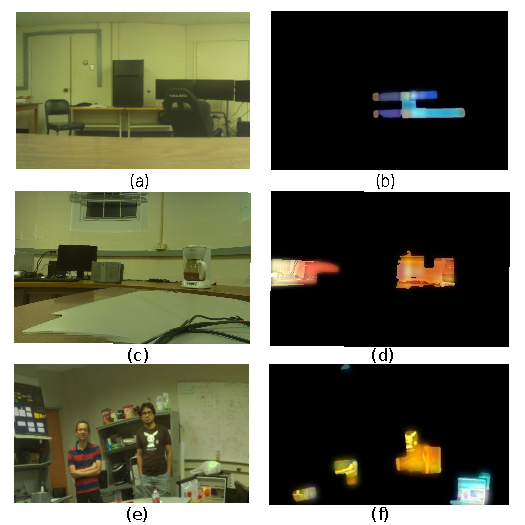
\epsfig{file=figs/Appliance.pdf,height=3in,width=3.2in} 
 	\label{fig:Object Detection}
 	\caption{Appliance and Object Detection Results}
 \end{figure}
 
 \begin{table}[t!]
 	\centering
 	\begin{tabular}{||p{1.8cm} | p{1.2cm} | p{1.2cm}| p{1cm} | p{1cm}||}
 		\hline
 		Event & Detected & Est. Temp. & Actual Temp & Location\\ [0.5ex]
 		\hline\hline
 		Heater ON  & Yes & 108 &  120 & LAB1\\
 		\hline
 		Fridge Open  & Yes & 98 &  100 & LAB1\\
 		\hline
 		Man 1 Standing  & Yes & 99 &  81 & LAB1\\
 		\hline
 		Man 2 Standing  & Yes & 103 &  83  & LAB1\\
 		\hline
 		Heater ON  & Yes & 110 &  120 & LAB2\\
 		\hline
 		Coffee ON  & Yes & 98 &  100 & LAB2\\
 		\hline
 		Fridge Open  & Yes & 98 &  100 & LAB2\\
 		\hline
 		Fridge \& Freezer Open  & No & 98 &  100 & LAB2\\
 		\hline
 		Man Hoodie  & No & 80 &  78 & LAB2\\
 		\hline
 		Man No-Hoodie & No & 80 &  78 & LAB2\\
 		\hline
 		Window Open & No & 78 &  75 & LAB2\\
 		\hline\hline
 	\end{tabular}
 	\label{table:DetectionTable}
 	\caption{Results Table}
 \end{table}


 There are three possible types of thermal regions in an image - background, cold region and hot region. The image that needs to be segmented is the stitched IR image and the objective is to create a thermal mask which separates the hot and cold regions from the background. Since the thermal image is being used for segmentation, the results are subject to the choice of color palette and range selection.  We ensure that the background has darker tones than the hot or cold surfaces which helps achieve the desired segmentation after image binarization using Otsu's method~\cite{Otsu}. We apply a 7$\times$7 neighborhood 2-D median filter to eliminate small blobs and get the few major thermal zones. The next step is to find the contour and their location of the blobs and then for each blob the average temperature is computed and the lookup (Table~\ref{table:temp}) is used to identify the object closest to that temperature. A pseudocode for the entire procedure has been given in Figure~\ref{algo:Two Object}.
 


    \subsection{Appliance State Detection/Energy Wasting Object Detection} 
    
    In this section we discuss the experiments performed using the mentioned methods for Appliance State Detect or Energy Wasting Object Detection. By an appliance state we mean an appliance turning ``ON'' and those who generate heat when turned ON. For example, the  Coffee-Maker and Heater both generate heat when turned ON. In Fig~\ref{fig:Object Detection}, we show that the Heater and Coffee-Maker and be distinctly distinguished as two hot sources when they are kept at a distance of about 2 feet apart. However the temperature value for both the appliances can vary in a range and distinguishing them using the particular lookup becomes difficult. 
    
   Discerning two definite thermal regions become difficult when they are in close proximity. For example in case of the Fridge-Freezer (Fig~\ref{fig:Object Detection}), the location is determined as cold zone as a whole and not separately as Fridge and Freezer. The open window in LAB 2 can not be detected as the difference between inside and outside temperature was low. In LAB 1, we took data for two humans and an open fridge and a heater turned 'ON' and all the objects could be detected as shown in Fig~\ref{fig:Object Detection}.
   

    
    
    
    
    \begin{figure}[t!]
    	\begin{center}
    		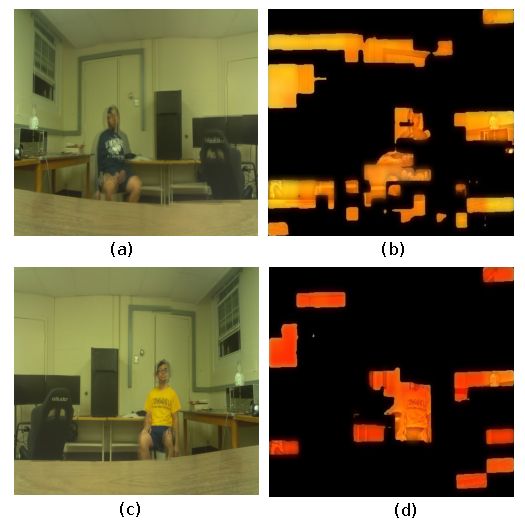
\epsfig{file=figs/Occupancy.pdf,height=2.in,width=2.5in}
    	\end{center}
    	\caption{Occupancy Detection Results}
    	\label{fig:Occupancy}
    \end{figure}
    
    
     \subsection{Occupancy Detection} 
     
     
     
     In this section we discuss the experiments performed for occupancy detection. Body heat can be detected through thermal imaging. Fig~\ref{fig:Occupancy} illustrates that two distinct human beings can be detected. However, for this technique to work the body temperature has to be significantly more than the background temperature. We donot consider the case where the room is much hotter than the body temperature as that is an improbable scenario. The temperature measured by the IR is the radiation from the human body. However this is subjected to variation - for example, we considered two cases where a human is wearing a hoodie and not wearing one in Fig~\ref{fig:Occupancy}. It was found that the one wearing hoodie has lower temperature than the other case. This creates a problem when the room temperature is close to that of the human body and detection of bodies is difficult. We found that its easier to identify a person in LAB 1 which has a colder temperature than in LAB 2, as LAB2 had poor air-conditioning and hence is warmer. 




 